\documentclass[main.tex]{subfiles}
\begin{document}
% neue TOC:
% \begin{itemize}
%     \item DONE wie im konzept gesagt vergleichen wir algorithmen um \$FRAGE zu beantworten
%     \item DONE zunächst definieren wir, wie und woran wir die performanz der algos vergleichen
%     \begin{itemize}
%         \item DONE Wir werden die performanz an 3 metriken messen: P,R,F1 (siehe BG section)
%     \end{itemize}
%     \item wie im konzept festgestellt, sind die pdas nicht vergleichbar. daher haben wir 2 verschiedene datensätze rausgesucht und oder erstellt:
%     \begin{itemize}
%         \item 2D 3D S: statisch, direkt ganze wolke da
%         \item FIN: dynamisch, inkrementell aufbauend
%     \end{itemize}
%     \item wir führen experimente auf beiden datensätzen durch 
%     \item im anschluss werten wir die ergebnisse aus und evaluieren inwiefern die algorithmen echtzeitfähig sind
% \end{itemize}

\chapter{Evaluation}

In diesem kapitel werden zuvor ausgewählte algorithmen einheitlich verglichen und die resultierenden ergebnisse ausgewertet.
\section{Protocol}
% \begin{itemize}
%     \item was wir zeigen wollen
%     \item daher vergleichen wir algorithmen
%     \item wie vergleichen wir, woran ziehen wir schlüsse? 
% \end{itemize}
This work aims to determine which plane detection algorithm is the most suitable for an AR/VR system. For this decision, we uniformly compare the algorithms selected in
Chapter~\ref{chap:Concept}. We split the comparison into two experiments conducted on different datasets: the 2D-3D-S and the
self-created FIN dataset. Since both datasets are fundamentally different, we will perform the experiments and the analysis separately and then compare the results.
First, we present the metrics used for comparison, followed by an outline of the used configurations of parameters for each experiment.
% In this work, we perform a uniform comparison of plane detection algorithms. This comparison aims to evaluate the real-time plane 
% detection on off-the-shelf hardware through the selection of the best algorithm.
% In the following subsection, we present the metrics used for the evaluation.
% We conduct experiments on both datasets and compare the results of both experiments with respect to the real-time applicability of the
% algorithms. Particularly interesting are the differences resulting from the temporal component.
% Finally, by evaluating the results of both experiments, we determine the most suitable plane detection algorithm for real-time, indoor environments. 

\subsection{Metrics}
\label{subsec:metrics}
To quantify the accuracy of the plane detection algorithms, we use the detected planes and the created ground truth to calculate the three following
metrics: Precision, Recall, and the F1-score. The procedure of calculation is taken from~\cite[Section~4]{Araújo_Oliveira_2020} and detailed
in Section~\ref{sec:metrics}.


\textcolor{red}{hier noch mehr ins detail gehen? (antwort) \underline{\hspace{2cm}}}


In addition to the accuracy of an algorithm, we precisely measure the calculation time by splitting the calculation into pre-processing, plane
detection, and post-processing.
RSPD and OPS perform an initial estimation of normals, while 3D-KHT and OBRG construct an octree during their
pre-processing phase. Note that the octree construction of OBRG includes a local estimation of normals on the
leaf level. OPS merges smaller planes if they pass a coplanarity test and then re-estimates the normals of the
resulting plane. In the post-processing step, OBRG refines the borders of detected planes by inserting
previously unallocated regions.
The pre-and post-processing steps are summarized in Table~\ref{tab:pre-post}.

\textbf{\textcolor{red}{\#detected planes als metrik einführen? ist imho wenig aussagekräftig da die GT erstellung so subjektiv ist}}

\begin{table}[H]
    \centering
    \begin{tabular}{c|cccc}
             & RSPD        & OPS        & 3D-KHT         & OBRG           \\ \hline
        Pre  & Normal est. & Normal est & Octree constr. & Octree constr. \\
        Post & /           & Merge      & /              & Refinement
    \end{tabular}
    \caption{Pre-processing and post-processing steps of the plane detection algorithms. RSPD and 3D-KHT do not have any post-processing steps.}
    \label{tab:pre-post}
\end{table}


\subsection{Parameterization of Algorithms}
Because the datasets inherit different amounts of noise, it is necessary to modify the algorithms accordingly.
We thereby modify the algorithms' parameterization to achieve more noise robustness.
In the following, the parameterizations of the algorithms with respect to the two experiments are outlined.
Therein, we refer to the parameterization of the 2D-3D-S experiment as the default configuration.
All deviations from this default configuration necessary for the FIN experiment are determined empirically.


\subsubsection{RSPD}
\textbf{\textcolor{red}{die abkürzungen werden sicherlich im BG erklärt.}}
\begin{table}[H]
    \centering
    \begin{tabular}{c|cccccc}
        Experiment & $l_O$ & $\varepsilon$ & MOR  & $k$ & MND & MDP   \\ \hline
        2D-3D-S    & 10    & 30            & 25\% & 30  & 60° & 0.258 \\
        FIN        & 10    & 30            & 25\% & 30  & 60° & 0.258
    \end{tabular}%
    \caption{Parameter configuration of RSPD used for the experiments.}
    \label{tab:rspd-param}
\end{table}

% FIXME overwork this paragraph given the newly obtained knowledge.
\paragraph{2D-3D-S}
For the 2D-3D-S experiment, we use the parameters of the provided implementation. These parameters include the maximum octree level $l_O$,
the minimum number of samples per leaf node $\varepsilon$, the maximum percentage of outliers per plane $\theta_{outlier}$, and
the size of the nearest neighborhood $k$. Note that while $k=50$ is used in the respective paper~\cite[Section~3.3]{Araújo_Oliveira_2020},
we use $k=30$ because, in our experience, it produces sufficient results while reducing the pre-processing time.

\paragraph{FIN}
\textbf{\textcolor{red}{Da bei der erstellung von rspd besonders auf noise resistenz geachtet wurde, passen wir keinen parameter für
        das FIN experiment an.
        Es wurden diverse anpassungen getestet, keine davon haben jedoch die ergebnisse verbessert.}}
\subsubsection{OPS}

\textcolor{red}{ja, die parameter werden im background \textit{sicherlich} erklärt}
\begin{table}[H]
    \centering
    \begin{tabular}{c|ccccc}
        Experiment & $\alpha_s$ & $KNN$       & $\theta_{h}$  & $\theta_{N}$ & $p$  \\ \hline
        2D-3D-S    & 3\%        & 30          & 0.05          & 100          & 0.99 \\
        FIN        & 3\%        & \textbf{90} & \textbf{0.35} & 100          & 0.99
    \end{tabular}%
    \caption{Parameter configuration of OPS used for the experiments.}
    \label{tab:ops-param}
\end{table}

\paragraph{2D-3D-S}
The parameter configuration used for the 2D-3D-S experiment is shown in the first row of Table~\ref{tab:ops-param}.
We use a sampling rate $\alpha_s$ of 3\% and a neighborhood $KNN$ of 30 for the estimation of normal vectors.
Additionally, we use a distance threshold $\theta_h$ of 0.05(m).
Furthermore, we set the inlier threshold $\theta_N$ to 100 and the probability for adaptively determining RANSAC iterations
$p$ to $0.99$, as proposed in~\cite[Section~4A]{Sun_Mordohai_2019}.

\paragraph{FIN}
For the FIN experiment, we increase $KNN$ to 90, as larger neighborhood sizes increase the accuracy of normal estimation and,
consequently, the overall accuracy of a method.
Furthermore, we increase the tolerated plane thickness $\theta_h$ because an increase in sensor noise ultimately thickens the recorded planes.
Both modifications are highlighted in bold in the second row of Table~\ref{tab:ops-param}.

\subsubsection{3D-KHT}
\begin{table}[H]
    \centering
    \begin{tabular}{c|ccccccc}
        Experiment & $\phi_{num}$ & $\rho_{num}$ & $s_{level}$ & $s_{ps}$ & $d_{max}$    & $s_\alpha$ & $s_\beta$ \\ \hline
        2D-3D-S    & 30           & 200          & 2           & 0.002    & 0.08         & 18         & 6         \\
        FIN        & 30           & \textbf{100} & 2           & 0.002    & \textbf{0.1} & \textbf{8} & 6
    \end{tabular}%
    \caption{Parameter configuration of 3D-KHT used for the experiments.}
    \label{tab:3dkht-param}
\end{table}

\paragraph{2D-3D-S}
The parameter configuration is shown in Table~\ref{tab:3dkht-param}. We use an accumulator discretization of 30 and 200 for $\phi$ and $\rho$, respectively.
Starting to check for planarity at an octree level $s_{level}$ of 2 seems to yield the best results.
\citeauthor{Limberger_Oliveira_2015}~\cite{Limberger_Oliveira_2015} propose
a minimum of 30 samples per cluster, however, we use $0.2\%$ of the total point cloud due to the wide ranges of point cloud sizes in the dataset (see Subsection~\ref{subsec:bg-stanford}).
Lastly, we set $s_\beta$ to 6, as proposed in~\cite[Section~3.1]{Limberger_Oliveira_2015}. In contrast, using a $s_\alpha$ value of 18 seemed to yield better results than the proposed 25.
% FIXME im background sicher gehen dass ich die erklärt habe

\paragraph{FIN}
For the FIN experiment, we modify the values of $\rho_{num}$, $d_{max}$ and $s_\alpha$ to accommodate for the higher levels of noise.
Reducing $\rho_{num}$ should decrease the accuracy, however, it seems to yield better results in a high-noise environment like the FIN dataset.
We increase $d_{max}$ and decrease $s_\alpha$ to allow for slightly thicker, e.g. noisier, planes to be detected.
The modification of parameters is highlighted in bold in Table~\ref{tab:3dkht-param}.

\subsubsection{OBRG}
\begin{table}[H]
    \centering
    \begin{tabular}{c|cccccc}
        Experiment & $l_{max}$ & $\theta_{res}$ & $\theta_{d}$ & $\theta_{ang}$ & $\theta_M$ & $\theta_p$    \\ \hline
        2D-3D-S    & 5         & 0.08           & 0.08         & 0.18           & 5000       & 90\%          \\
        FIN        & 5         & \textbf{0.22}  & \textbf{0.2} & \textbf{0.2}   & 5000       & \textbf{70\%}
    \end{tabular}
    \caption{Parameter configuration of OBRG used for the experiments.}
    \label{tab:obrg-param}
\end{table}

% FIXME boldness in tables in der caption erläutern

\paragraph{2D-3D-S}
The used configurations for the experiments are shown in Table~\ref{tab:obrg-param}.
Due to the low level of noise, we assign a very small tolerance to $\theta_{res}$ and $\theta_d$. Additionally, we assign a high
planarity threshold value of $\theta_p = 90\%$.

\paragraph{FIN}
Due to higher levels of noise, and thus, thicker walls, we increase the residual threshold $\theta_{res}$, the distance
threshold $\theta_d$, and the angular divergence threshold $\theta_{ang}$. According to~\cite[Section~3.4]{Vo_Truong-Hong_Laefer_Bertolotto_2015},
the planarity threshold $\theta_p$ should be chosen between 70\% and 90\% depending on the noise level. As the expected noise level of the
FIN dataset is much higher than the noise of the 2D-3D-S dataset, we reduce this threshold to 70\%.
The used parameters for the FIN experiment are summarized in the second row of Table~\ref{tab:obrg-param}.


\section{Results}
This section deals with the results of the experiments. The individual results of both experiments are presented and analyzed.

was ich sagen möchte:
\begin{itemize}
    \item bei p,r,f1 zeigt sich ein muster
          \begin{itemize}
              \item OPS hat die beste präzision, RSPD dominiert bei recall und F1
              \item RSPD und 3D-KHT haben die besten $t_{calc}$ werte
          \end{itemize}
    \item \textbf{\textcolor{red}{das folgende in die Conclusion:}}
    \item bei FIN ist aufgrund der preproc zeit von rspd nur 3dkht echtzeitfähig.
          \begin{itemize}
              \item manche kameras, beispielsweise die intel realsense, können mittlerweile normalen mitliefern
              \item daher sehen wir rspd als echtzeitfähig an, unter der voraussetzung dass die normalen spätestens beim SLAM schritt vorhanden
                    sind (siehe~\ref{fig:concept})
          \end{itemize}
\end{itemize}

\subsection{2D-3D-S}

Wir haben RSPD, OPS, 3D-KHT und OBRG auf 139 Scenen des 2D-3D-S Datensatzes laufen lassen. Im Anschluss wurden zu jeder Scene die Präzision,
der Recall und der F1-Score von jedem Algorithmus berechnet. Dazu wurden die Berechnungszeiten gemessen und in pre-processing, plane detection und
post-processing aufgeteilt. Table~\ref{tab:res-3d2ds-total} zeigt die average der berechneten Ergebnisse zu jedem Algorithmus. Durch dicke Schrift
werden die besten durchschnittswerte hervor gehoben. Dazu sei anzumerken, dass kein bester wert von $t_{post}$ angedeutet wird, da zwei der algorithmen
keine post-processing schritte haben und daher "per default" weniger zeit in diesem Schritt verbringen.

\begin{table}[H]
    \centering
    \begin{tabular}{c|cccccc}
        Algorithm & Precision        & Recall           & F1-Score         & $t_{pre}$    & $t_{calc}$    & $t_{post}$ \\ \hline
        RSPD      & 86.22\%          & \textbf{89.31\%} & \textbf{87.40\%} & 109.94       & \textbf{1.63} & /          \\
        OPS       & \textbf{90.66\%} & 71.21\%          & 79.09\%          & 16.90        & 8.99          & 0.35       \\
        3DKHT     & 71.41\%          & 75.26\%          & 72.87\%          & \textbf{1.2} & 1.71          & /          \\
        OBRG      & 83.15\%          & 62.77\%          & 69.46\%          & 47.25        & 39.85         & 2.89
    \end{tabular}
    \caption[Overall 2D-3D-S Results]{Average results of each algorithm over the 2D-3D-S dataset. The right half of the columns shows the average time spent in
        pre-processing ($t_{pre}$), the average time spent in the plane detection ($t_{calc}$), and the average time spent in post-processing steps ($t_{post}$).
        Note, that the absence of post-processing steps is denoted as "/". All times are measured in seconds.}
    \label{tab:res-3d2ds-total}
\end{table}

\textbf{\textcolor{red}{das aufteilen macht zwar semantisch sinn, ist aber uncool für den leseflow glaube ich }}

\paragraph{Accuracy}
Mit einer Präzision von 86\%, einem Recall von 89\% und einem F1-Score von 87\% ist RSPD der insgesamt präziseste algorithmus. OPS übertrifft RSPD zwar
in der Precision mit einem Wert von ca. 90\%, erzielt dafür aber deutlich schlechtere Recall und F1-Score ergebnisse.
3D-KHT erzielt durchschnittliche Ergebnisse mit einer Precision, Recall und F1-Score im unteren Bereich der 70\%.
Mit einer guten Präzision von ca. 83\% aber dafür vergleichsweise schlechten Recall und F1-Score Werten liefert OBRG die insgesamt schlechtesten
Accuracy Ergebnisse des 2D-3D-S Experiments.

\paragraph{Time}
While RSPD takes the longest during pre-processing, it also spends the shortest amount of time in the plane detection phase.
The algorithm that takes the total shortest average time is 3D-KHT with a cumulated average of just under 3 seconds.
Both OPS and OBRG spend multiple seconds during pre-processing, plane detection, and, in the case of OBRG, also during post-processing steps.
The average post-processing time of OBRG takes, on average, about as long as 3D-KHT takes in total.

\subsection{FIN}
Jeder der insgesamt 732 Zeitschritte des FIN Datensatzes wurde von jedem algorithmus verarbeitet. Im Anschluss wird 
jeder Zeitschritt seperat ausgewertet, also die Präzision, der Recall und der F1-Score berechnet. Dazu 
wurden, wie beim 2D-3D-S Experiment die Berechnungszeiten der Algorithmen für jeden Zeitschritt gemessen.  
Die durchschnittlichen Ergebnisse über alle Zeitschritte des FIN Experiments werden
in Table~\ref{tab:res-fin-total} präsentiert.

\begin{table}[H]
    \centering
    \begin{tabular}{c|cccccc}
        Algorithm & Precision        & Recall           & F1-Score         & $t_{pre}$     & $t_{calc}$    & $t_{post}$ \\ \hline
        RSPD      & 57.30\%          & \textbf{60.75\%} & \textbf{58.70\%} & 14.36         & \textbf{0.19} & /          \\
        OPS       & \textbf{69.38\%} & 29.23\%          & 39.43\%          & 4.61          & 0.89          & 0.13       \\
        3DKHT     & 49.76\%          & 44.40\%          & 46.48\%          & \textbf{0.14} & 0.29          & /          \\
        OBRG      & 49.23\%          & 27.42\%          & 33.94\%          & 6.03          & 14.70         & 0.35
    \end{tabular}
    \caption[Overall 2D-3D-S Results]{Average results of each algorithm over the FIN dataset. The right half of the columns shows the average time spent in
        pre-processing ($t_{pre}$), the average time spent in the plane detection itself ($t_{calc}$), and the average time spent in post-processing steps ($t_{post}$).
        Note, that the absence of post-processing steps is denoted as "/".}
    \label{tab:res-fin-total}
\end{table}

\paragraph{Accuracy}
OPS hat mit nahezu 70\% die höchste Präzision der Algorithmen. RSPD hat dafür mit ca. 60\% jeweils die besten
Werte für Recall und F1-Score erzielt. 3D-KHT und OBRG erzielen ähnliche Ergebnisse der precision, bei Recall und 
F1-Score ist 3D-KHT jedoch um durchschnittlich 15\% besser als OBRG.

\paragraph{Time}
Nachdem RSPD die durschnittlich meiste Zeit im pre-processing verbringt, wird im Anschluss am wenigsten 
Zeit in der plane detection Phase verbracht. Insgesamt braucht 3D-KHT mit $0.34s$ jedoch am kürzesten für die Berechnung 
eines Zeitschritts. OPS erzielt mit ca. 5 sekunden vergleichsweise durchschnittliche Zeiten und OBRG 
braucht mit mehr als 20 sekunden insgesamt am längsten für die Berechnung eines Zeitschritts.

\textbf{\textcolor{red}{might be more appropriately placed somewhere above}}
Die Punktwolken des FIN experiments wachsen inkrementell. Unter der Annahme, dass dieses Wachstum stetig ist,
würden die durschnittswerte der Berechnungszeiten eines nicht-exponentiellen algorithmuses eher die Berechnungszeit
der Punktwolke an Zeitschritt $t_{max} \cdot \frac{1}{2}$ beschreiben.
Es ist daher sinnvoll, den zusammenhang zwischen der größe der Punktwolke und der Berechnungszeit zu betrachten.
In Figure~\ref{fig:dynhallway} werden die Dauer der Berechnung jedes Zeitschritts der Dateigröße von der
 \textit{hallway} Scene des FIN Datensatzes gegenüber gestellt. 

\begin{figure}[H]
    \centering
    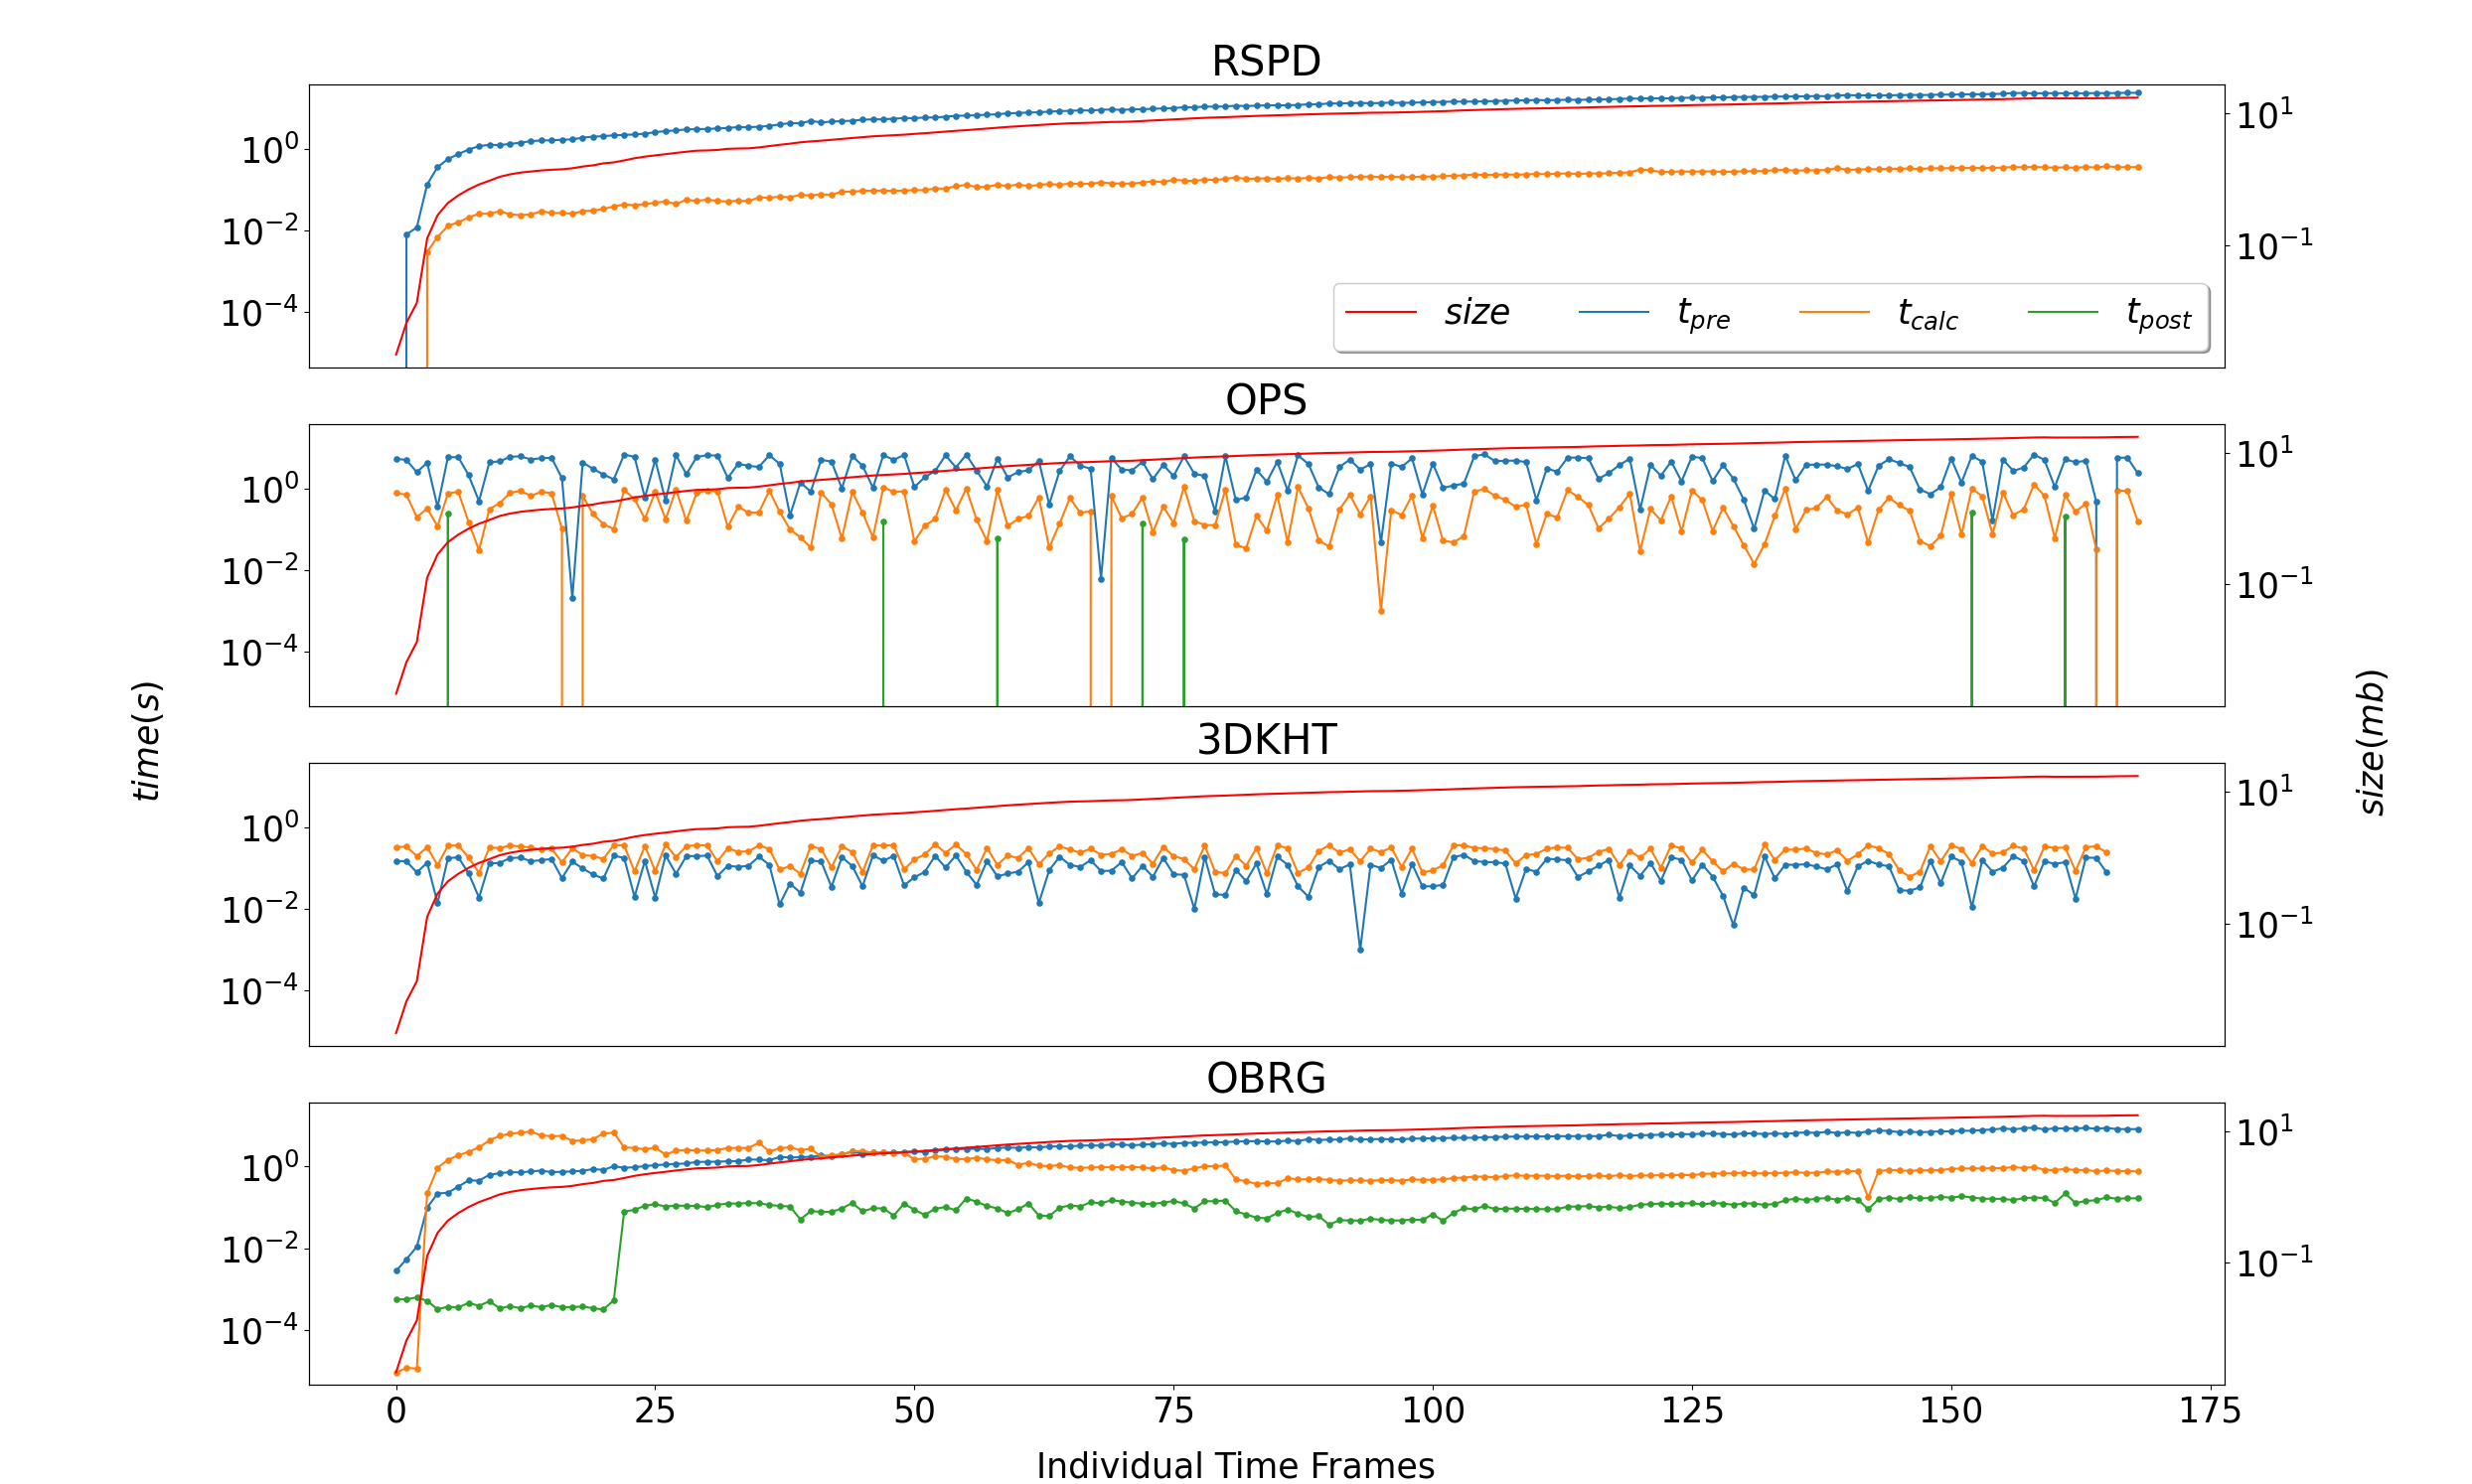
\includegraphics[width=\textwidth]{images/dyn_time-hallway.png}
    \caption[Time Results Hallway]{Time spent in pre-processing (blue), plane detection (yellow), and post-processing 
    (green) of the hallway scene and cloud sizes (red) of each time step.}
    \label{fig:dynhallway}
\end{figure}

Bei RSPD und OBRG kann man direkt sehen, dass die pre-processing zeiten $t_{pre}$ proportional zur größe der punktwolke
 sind. Im kontrast dazu scheinen bei OPS und 3D-KHT die pre-processing zeiten mehr mit den Zeiten der plane detection 
 $t_{calc}$ in Verbindung zu stehen. Bei RSPD, OPS und 3D-KHT scheint $t_{calc}$ unabhängig von der Größe der Punktwolke 
 zu sein und befindet sich stets unter einem gewissen Wert. Einzig auffallend ist das rapide Wachstum von OBRG im zeitraum
 vom Start bis ca. 25.  



\subsection{Comparison}
When comparing Table~\ref{tab:res-3d2ds-total} and Table~\ref{tab:res-fin-total}, a pattern emerges:
OPS has the highest precision with ca. 90\% and ca. 69\%, RSPD scores the best Recall and F1-Score values, and 3D-KHT has the lowest total
processing time.

Reiterating our definition of real-time of Section~\ref{sec:realtime}, we consider an algorithm to be real-time-applicable if its calculation time is below one second.
Given the results of the 2D-3D-S experiment, none of the algorithms is real-time applicable, as even the quickest algorithm, 3D-KHT, takes
an average of ca. 3 seconds per calculation.
However, the entire environment would not be available from the start in a real-life scenario. The FIN experiment represents a more realistic
view on the processing times due to the incrementally growing point cloud. \textbf{\textcolor{red}{in Grafik N kann man den zusammenhang
        von größe der punktwolke und berechnungszeit ablesen. (TODO)}}

\section{Summary}

\textbf{\textcolor{red}{im not sure where exactly to put this}}
\begin{itemize}
    \item bei 2D-3D-S ist kein algorithmus echtzeitfähig
          \begin{itemize}
              \item Da aber niemals die komplette wolke direkt vorhanden ist sagt das nicht viel aus
              \item aussagekräftiger ist daher der zusammenhang zwischen zeit und größe der punktwolke
              \item daher sind p,r,f1 von größerem interesse für den vergleich zwischen 2D-3D-S und FIN
          \end{itemize}
\end{itemize}


% NOTE 3DKHT kann keine löcher oder non-rectangular ebenen basteln!
This section combines the preceding results of both experiments.
RSPD is the only algorithm that produces comparable results to the Stanford experiment in the dynamic experiment.
The remaining algorithms cannot reliably detect planes in an incrementally growing environment inheriting varying degrees of noise.

The reason for RSPD's dominance is likely caused by the inherent robustness against noise, as described in Section~

Die ergebnisse der beiden experimente unterscheiden sich in folgendem punkt. Dazu sei gesagt, dass die experimente folgende übereinstimmungen haben.
Das lässt sich so erklären. Alternative gründe davon könnten diese hier sein.

Ich denke RSPD ragt heraus, da hier besonders auf noise resistenz geachtet wurde. % TODO verweis auf diverse noise tests im BG


\end{document}